\documentclass{article}
\usepackage{amssymb}
\usepackage{amsmath}
\usepackage[left=1in,right=1in,top=.8in,bottom=.8in]{geometry}
\usepackage{graphicx}
\parindent=0in
\begin{document}
Imran Yafai\\
Computational Physics\\
Project 6B\\
\\
Closed form solution for circuit:\\
Capacitor Charged to Initial Voltage of 5V with Capacitance 3 F connected to an 8$\Omega$ Resistor
\begin{figure}[ht!]
\centering
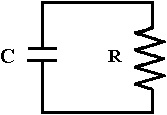
\includegraphics[width=30mm]{circuit.jpg}
\caption{High-Quality Circuit Diagram}
\label{overflow}
\end{figure}\\
Voltage Drop over Resistor:
\[V_R=I_RR\]
Charge on Capacitor:\\
\[Q_C=V_CC\]
\[V_R=\frac{dQ}{dt}R\]
This current entering the resistor, is the negative of current leaving the capacitor\\
\[V_R=-\frac{dQ_C}{dt}R\]
Subsituting for $V_R$ and rewritting $Q_C$ as Q
\[\frac{Q}{RC}=-\frac{dQ}{dt}\]
This can be rewritten as
\[-\frac{dQ}{Q}=\frac{dt}{RC}\]
And then we integrate the from time 0 to .5 s
\[\int_{Q_0}^{Q_f} -\frac{dQ}{Q}=\int_0^{t_f}\frac{dt}{RC}\]
This gives us:
\[-\ln(Q)\bigg|_{Q_0}^{Q_f}=\frac{1}{RC}t\bigg|_0^{t_f}\]
\[\ln{Q_0}-\ln{Q_f}=\ln{\frac{Q_0}{Q_f}}=\frac{t_f}{RC}\]
This equation can be rewritten as
\[\frac{Q_0}{Q_f}=e^{t_f/RC}\]
and so the charge on the capacitor at .5 seconds is
\[Q_f=Q_0e^{-t_f/RC}=(3*5)e^{-.5/8*3} \mathrm{\,C}= \mathrm{14.69073272 \,C}\]
\end{document}